\problemname{Lateral Damage}

\newcommand{\maxn}{100}
\newcommand{\maxk}{10}
\newcommand{\maxq}{2500}

\illustration{0.3}{battleships.jpg}{
    The original \emph{Battleships} game, \\
    before the upgrade to a $\maxn \times \maxn$ grid. \\
    CC BY-NC 3.0 by Pavel Ševela on \href{https://commons.wikimedia.org/wiki/File:Hra_n\%C3\%A1mo\%C5\%99n\%C3\%AD_bitva_(1).jpg}{Wikimedia Commons}
}%
You are playing \emph{Battleships} in a large ocean with large ships.
More precisely, there is a large square grid of size at most $\maxn\times \maxn$
and inside it are up to $\maxk$ of the largest type of ship in Battleships
-- the aircraft carrier -- which has a length of five tiles,
placed either horizontally or vertically.
The ships do not overlap, but they are allowed to be adjacent to each other.
See Figure~\ref{fig:carriers} for an example.

Unfortunately, your opponent appears to bend the rules to their liking,
and does not always determine the placement of their ships before you start shooting.
You are not impressed by their attempt at cheating, and decide to try and win the game anyway.

\begin{figure}[!h]
    \centering
    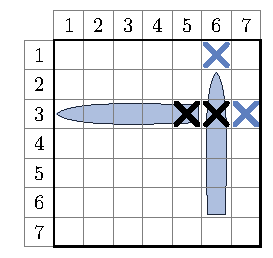
\includegraphics[width=0.29\textwidth]{sample}
    \caption{Illustration of Sample Interaction 1 after the first four shots were fired.}
    \label{fig:carriers}
\end{figure}

Your goal is to locate and sink all your opponent's aircraft carriers in at most $\maxq$ shots,
that is, you must hit each of the five tiles of all their ships.

\begin{Interaction}
    This is an interactive problem.
    Your submission will be run against an \emph{interactor},
    which reads from the standard output of your submission
    and writes to the standard input of your submission.
    This interaction needs to follow a specific protocol:

    The interactor first sends
    one line with two integers $n$ and $k$ ($5 \le n \le \maxn$, $1 \le k \le \maxk$),
    the size of the grid and the number of ships.
    It is guaranteed that it is possible to place $k$ aircraft carriers in the grid without overlap.

    Then, your program needs to start firing shots.
    Each shot is fired by printing one line of the form ``\texttt{$x$~$y$}'' ($1 \le x,y \le n$),
    indicating you shoot at position $(x, y)$.
    The interactor will respond with ``\texttt{hit}'' if the shot was a hit,
    ``\texttt{sunk}'' if the shot caused an aircraft carrier to sink, and ``\texttt{miss}'' otherwise.
    If you have shot the same location before,
    the response will be ``\texttt{miss}''.

    Once you sink the last aircraft carrier,
    the interaction will stop and your program must exit.

    The interactor is adaptive:
    the placement of the ships may be determined during the interaction,
    and may depend on where you decide to shoot.
    It is guaranteed that the final placement of the ships
    will be consistent with the responses to all your shots.

    Make sure you flush the buffer after each write.

    A testing tool is provided to help you develop your solution.

    Firing more than $\maxq$ shots will result in a wrong answer.
\end{Interaction}
